%\documentclass[12pt,draft]{article}
\documentclass[12pt]{article}
\usepackage{CJK}
\usepackage{mathrsfs}
\usepackage{amsmath,amsthm,amsfonts,amssymb}
\usepackage{geometry}
\usepackage{fancyhdr}
\usepackage{indentfirst}
\usepackage{float}
\usepackage[dvips]{graphicx}
\usepackage{subfigure}
\usepackage[font=small]{caption}
\usepackage{threeparttable}
\usepackage{cases}
\usepackage{multicol}
\usepackage{url}
\usepackage{amsmath}
\usepackage{bm}
\usepackage{xcolor}
\usepackage{overpic}
\usepackage[round]{natbib}
\usepackage[utf8]{inputenc}
\usepackage[american]{babel}
\usepackage{graphicx}
\usepackage{algorithm, algorithmicx, algpseudocode}
\numberwithin{equation}{section}
\geometry{left=1.5cm,right=1.5cm,top=1.5cm,bottom=1.5cm}
\setlength{\parskip}{0.3\baselineskip}
\setlength{\headheight}{15pt}
\usepackage{color}   %May be necessary if you want to color links
\usepackage{hyperref}
\hypersetup{
    colorlinks=true, %set true if you want colored links
    linktoc=all,     %set to all if you want both sections and subsections linked
    linkcolor=blue,  %choose some color if you want links to stand out
}
\setcounter{secnumdepth}{4}
\begin{document}\small
\title{Deep Learning\citep{Goodfellow-et-al-2016-Book} Notes}
\author{Yan JIN}
\pagestyle{fancy}\fancyhf{}
\lhead{}\rhead{JIN Yan}
\lfoot{\textit{}}\cfoot{}\rfoot{\thepage}
\renewcommand{\headrulewidth}{1.pt}
\renewcommand{\footrulewidth}{1.pt}
\maketitle
\tableofcontents
%=======================================
\section{Matrix Derivative} \par
Here we choose \textbf{Numerator layout}. \par
\textbf{Scalar}: x, y; \par
\textbf{Vector}:\par
\begin{equation}
	\mathbf{x} = 
	\begin{bmatrix}
		x_1\\ x_2\\ \vdots\\ x_3\\
	\end{bmatrix}, 
	\mathbf{y} = 
	\begin{bmatrix}
		y_1\\ y_2\\ \vdots\\ y_3\\
	\end{bmatrix};	
\end{equation}\par
\textbf{Derivatives with Vectors}:
\begin{equation}
	\nabla_{x} \mathbf{y} = \frac{\partial \mathbf{y}}{\partial x} =
	\begin{bmatrix}
		\frac{\partial y_1}{\partial x}\\
		\frac{\partial y_2}{\partial x}\\
		\vdots\\
		\frac{\partial y_n}{\partial x}\\
	\end{bmatrix},
	\nabla_{\mathbf{x}} y = \frac{\partial y}{\partial \mathbf{x}} =
	\begin{bmatrix}
		\frac{\partial y}{\partial x_1},
		\ \ \frac{\partial y}{\partial x_2},
		\ \ \cdots,
		\ \ \frac{\partial y}{\partial x_n}\\
	\end{bmatrix},
	\nabla_{\mathbf{x}} \mathbf{y} = \frac{\partial \mathbf{y}}{\partial \mathbf{x}} =
	\begin{bmatrix}
		\frac{\partial y_1}{\partial x_1} & \frac{\partial y_1}{\partial x_2} & \cdots & \frac{\partial y_1}{\partial x_n}\\
		\frac{\partial y_2}{\partial x_1} & \frac{\partial y_2}{\partial x_2} & \cdots & \frac{\partial y_2}{\partial x_n}\\
		\vdots & \vdots & \ddots & \vdots\\
		\frac{\partial y_m}{\partial x_1} & \frac{\partial y_m}{\partial x_2} & \cdots & \frac{\partial y_m}{\partial x_n}\\
	\end{bmatrix};
\end{equation} \par
In vector calculus, the derivative of a vector function $\mathbf{y}$ with respect to a vector $\mathbf{x}$ whose components represent a space is known as the \textbf{Jacobian matrix}. \par
\textbf{Derivatives with Matrices}:
\begin{equation}
	\frac{\partial \mathbf{Y}}{\partial x} =
	\begin{bmatrix}
		\frac{\partial y_{11}}{\partial x} & \frac{\partial y_{12}}{\partial x} & \cdots & \frac{\partial y_{1n}}{\partial x}\\
		\frac{\partial y_{21}}{\partial x} & \frac{\partial y_{22}}{\partial x} & \cdots & \frac{\partial y_{2n}}{\partial x}\\
		\vdots & \vdots & \ddots & \vdots\\
		\frac{\partial y_{m1}}{\partial x} & \frac{\partial y_{m2}}{\partial x} & \cdots & \frac{\partial y_{mn}}{\partial x}\\
	\end{bmatrix},
	\frac{\partial y}{\partial \mathbf{X}} =
	\begin{bmatrix}
		\frac{\partial y}{\partial x_{11}} & \frac{\partial y}{\partial x_{21}} & \cdots & \frac{\partial y}{\partial x_{p1}}\\
		\frac{\partial y}{\partial x_{12}} & \frac{\partial y}{\partial x_{22}} & \cdots & \frac{\partial y}{\partial x_{p2}}\\
		\vdots & \vdots & \ddots & \vdots\\
		\frac{\partial y}{\partial x_{1q}} & \frac{\partial y}{\partial x_{2q}} & \cdots & \frac{\partial y}{\partial x_{pq}}\\
	\end{bmatrix};
\end{equation} \par
The \textbf{directional derivative} of a scalar function $f(\mathbf{x})$ in the direction of the unit vector $\mathbf{u}$ is the slope of the function f in direction $\mathbf{u}$: \par
	\begin{equation}
		\nabla_{\bold{u}}{f}(\bold{x}) = [\frac{\partial}{\partial \alpha}f(\bm{x}+\alpha \bm{u})]|_{\alpha=0}
		=\sum_{i=1}^{n}\frac{\partial f}{\partial x_i}u_i=\frac{\partial f}{\partial \mathbf{x}}\mathbf{u}
	\end{equation}
%=======================================
\section{Chapter 2 Linear Algebra}
%\addcontentsline{toc}{subsection}{Singular Value Decomposition (\$2.8)}
\subsection{Singular Value Decomposition (\$2.8)}
SVD(Singular Value Decomposition):
\begin{equation}
	\mathbf{A=UDV}^{T}
\end{equation}
\textbf{A}: m x n matrix; \textbf{U}: m x m matrix; \textbf{D}: m x n matrix;  \textbf{V}: n x n matrix; \par
\textbf{U} and \textbf{V} are orthogonal; \textbf{D} is diagonal but not necessarily square.\par
The elements along the diagonal of \textbf{D} are \emph{singular values} of \textbf{A};
The columns of \textbf{U} are the \emph{left-singular vectors}, the columns of \textbf{V} are the \emph{right-singular vectors} \par
The left-singular vectors are the eigenvectors of $\mathbf{AA}^T$; the right-singular vectors are the eigenvectors of $\mathbf{A}^T\mathbf{A}$ \par
Every real matrix has a SVD. One of the usage of SVD is to generalize matrix inversion to non-square matrices.
%-----------------------------------------
\subsection{Example Principal Components Analysis (\$2.12)}
Inputs: A collection of m points \{$\mathbf{x}^{(1)},...,\mathbf{x}^{(m)}$\} in $\mathbb{R}^{n}$. \par
Target is to lossy compression to these points, that means to storing the points in a way that requires less memory but may lose some precision. We would like to lose as little precision as possible. So, \par
Outputs: For each point $\mathbf{x}^{(i)} \in \mathbb{R}^{n}$ we will find:
\begin{enumerate}
	\item A $\mathbf{c}^{(i)} \in \mathbb{R}^{l}$, where $l < n$;
	\item A encoding function: $f(\mathbf{x})=\mathbf{c}$; 
	\item A decoding function: $\mathbf{x} \approx g(f(\mathbf{x}))$.
\end{enumerate}
%=======================================
\section{Chapter 3 Probability and Information Theory}
\subsection{Expectation, Variance and Covariance}
\begin{equation}\begin{split}
	Expectation: \mathbb{E}_{X \sim P}[f(x)]&=\int p(x)f(x)dx \\
	Variance: Var(f(x))&=\mathbb{E}[(f(x)-\mathbb{E}[f(x)])^2] \\
	Covariance: Cov(f(x),g(x))&=\mathbb{E}[(f(x)-\mathbb{E}[f(x)])(g(x)-\mathbb{E}[g(x)])]
\end{split}\end{equation}
%=======================================
\section{Chapter 5 Machine Learning Basics}
\subsection{Estimators, Bias and Variance (\$5.4)}
\subsubsection{Point Estimation}
\subsubsection{Bias}
\begin{equation}
	bias(\hat{{\boldsymbol\theta}}_m)=\mathbb{E}(\hat{\boldsymbol\theta}_m)-\boldsymbol\theta
\end{equation}
Proof of formula (5.39):
\begin{equation}\begin{split}
	\hat{\mu}_m&=\mathbb{E}[x^{(i)}]=\frac{1}{m}\sum_{i=1}^{m}x^{(i)} \\
	\mu&=\mathbb{E}[\hat{\mu}_m] \\
	Var(x^{(i)})&=\mathbb{E}[(x^{(i)}-\mu)^2]=\sigma^2 \\
	Var(\hat{\mu}_m)&=\mathbb{E}[(\hat{\mu}_m-\mu)^2] =\frac{\sigma^2}{m}
\end{split}\end{equation}
so:
\begin{equation}\begin{split}
	\mathbb{E}[\hat{\sigma}^2_m]
	&=\mathbb{E}[\frac{1}{m}\sum_{i=1}^{m}(x^{(i)}-\hat{\mu}_m)^2] \\
	&=\frac{1}{m}\mathbb{E}[\sum_{i=1}^{m}(x^{(i)}-\mu+\mu-\hat{\mu}_m)^2] \\
	&=\frac{1}{m}\mathbb{E}[\sum_{i=1}^{m}(x^{(i)}-\mu)^2+2\sum_{i=1}^{m}(x^{(i)}-\mu)(\mu-\hat{\mu}_m)+\sum_{i=1}^{m}(\mu-\hat{\mu}_m)^2] \\
	&=\frac{1}{m}\mathbb{E}[\sum_{i=1}^{m}(x^{(i)}-\mu)^2+2m(\hat{\mu}_m-\mu)(\mu-\hat{\mu}_m)+m(\mu-\hat{\mu}_m)^2] \\
	&=\frac{1}{m}\mathbb{E}[\sum_{i=1}^{m}(x^{(i)}-\mu)^2-m(\hat{\mu}_m-\mu)^2] \\
	&=\frac{1}{m}(\sum_{i=1}^{m}\mathbb{E}[(x^{(i)}-\mu)^2]-m\mathbb{E}[(\hat{\mu}_m-\mu)^2]) \\
	&=\frac{1}{m}(mVar(x^{(i)})-mVar(\hat{\mu}_m)) \\
	&=Var(x^{(i)})-Var(\hat{\mu}_m) \\
	&=\sigma^2-\frac{\sigma^2}{m}=\frac{m-1}{m}\sigma^2
\end{split}\end{equation}
\subsubsection{Variance and Standard Error}
Variance:$ Var(\hat{\theta})$ \par
Standard Error: $SE(\hat{\theta})=\sqrt{Var(\hat{\theta})}$ \par
\subsubsection{Trading off Bias and Variance to Minimize Mean Square Error}
Proof (5.54):
\begin{equation}\begin{split}
	MSE&=\mathbb{E}[(\hat{\theta}_m-\theta)^2] \\
	&=\mathbb{E}[\hat{\theta}_m^2]-2\theta\mathbb{E}(\hat{\theta}_m)+\theta^2 \\
	Bias(\hat{\theta}_m)^2
	&=(\mathbb{E}[\hat{\theta}_m]-\theta)^2 \\
	&=\mathbb{E}[\hat{\theta}_m]^2-2\mathbb{E}[\hat{\theta}_m]\theta+\theta^2 \\
	Var(\hat{\theta}_m)
	&=\mathbb{E}[(\hat{\theta}_m-\mathbb{E}[\hat{\theta}_m])^2]\\
	&=\mathbb{E}[\hat{\theta}_m^2-2\hat{\theta}_m\mathbb{E}[\hat{\theta}_m]+\mathbb{E}[\hat{\theta}_m]^2]\\
	&=\mathbb{E}[\hat{\theta}_m^2]-\mathbb{E}[\hat{\theta}_m]^2\\
	\Rightarrow
	MSE&=Bias(\hat{\theta}_m)^2+Var(\hat{\theta}_m)
\end{split}\end{equation}
%=======================================
\subsection{Frequentist Statistics and Baysian Statistics ($\$5.5 \sim \$5.6$)}
Frequentist: Estimate a single value of $\boldsymbol\theta$, then making all predictions thereafter based on that \textbf{one} estimate; \par
Baysian: Consider \textbf{all} possible values of $\boldsymbol\theta$ when making a prediction; \par
Frequentist: The true parameter value $\boldsymbol\theta$ is \textbf{fixed but unknown}, while the point estimate $\hat{\boldsymbol\theta}$ is a random variable and a function of \textbf{the dataset}(which is seen as \textbf{random}); \par
Baysian: \textbf{Dataset} is directly observed and is \textbf{not random}; the true parameter value $\boldsymbol\theta$ is \textbf{unknown or uncertain} and thus is represented as a random variable; \par
Differences between MLE(Maximum Likelihood Estimation) and Bayesian estimation:
\begin{enumerate}
	\item MLE: Make predictions using a \textbf{point estimate} of $\boldsymbol\theta$; \par
	Bayesian: Using a \textbf{full distribution} over $\boldsymbol\theta$;
	\item MLE: Address the uncertainty on a given point estimate of $\boldsymbol\theta$ by evaluating its \textbf{variance}; \par
	Bayesian: Simply \textbf{integrate over it};
	\item Baysian: Use a priori, which expresses a preference for \textbf{simpler and smooth models}, and seems as a source of \textbf{subjective human judgment} impacting the predictions; \par
	\item Baysian: \textbf{Generalize much better} when training data is \textbf{small}, but \textbf{high computation cost} when training data is \textbf{large};
\end{enumerate}
%-----------------------------------------
\subsubsection{Frequentist Statistics - Maximum Likelihood Estimation (MLE)}
$p_{data}(\boldsymbol{x})$: \textbf{The true but unknown} data generating distribution. \par
 $\mathbb{X}=\{x^{(1)},...,x^{(m)}\}$: Drawn independently from $p_{data}(\boldsymbol{x})$. \par
$\hat{p}_{data}(\boldsymbol{x})$: The empirical distribution. \par
$p_{model}(\boldsymbol{x;\theta})$: A parametric family of probability distribution over the space indexed by $\boldsymbol{\theta}$ for estimating the $p_{data}(\boldsymbol{x})$. \par
The maximum likelihood estimator for $\boldsymbol{\theta}$:
\begin{equation}\begin{split}
	\boldsymbol{\theta_{ML}}&=\underset{\boldsymbol{\theta}}{argmax}\ p_{model}({\mathbb{X};		\boldsymbol{\theta}}) \\
	&=\underset{\boldsymbol{\theta}}{argmax}\prod_{i=1}^{m}p_{model}(x^{(i)};\boldsymbol{\theta}) \\
	&=\underset{\boldsymbol{\theta}}{argmax}\sum_{i=1}^{m}log\ p_{model}(x^{(i)};\boldsymbol{\theta}) \\
	&=\underset{\boldsymbol{\theta}}{argmax}\frac{1}{m}\sum_{i=1}^{m}log\ p_{model}(x^{(i)};\boldsymbol{\theta}) \\
	&=\underset{\boldsymbol{\theta}}{argmax}\ \mathbb{E}_{\boldsymbol{x}\sim\hat{p}_{data}}log\ p_{model}(\boldsymbol{x};\boldsymbol{\theta}) \\
\end{split}\end{equation} \par
MLE is an attempt to make the $p_{model}$ match $\hat{p}_{data}$, because we have no direct access to $p_{data}$.
%-----------------------------------------
\subsubsection{Baysian Statistics}
$p(\boldsymbol\theta)$: Prior probability distribution(the prior). \par
$\{x^{(1)},...,x^{(m)}\}$: Data samples. \par
We reform the belief about $\boldsymbol\theta$(the posterior $p(\boldsymbol\theta|x^{(1)},...,x^{(m)})$) by the data likelihood $p(x^{(1)},...,x^{(m)}|\boldsymbol\theta)$ and the prior $p(\boldsymbol\theta)$ via \textbf{Bayes' rule}: 
\begin{equation}
	p(\boldsymbol\theta|x^{(1)},...,x^{(m)})=\frac{p(x^{(1)},...,x^{(m)}|\boldsymbol\theta)p(\boldsymbol\theta)}{p(x^{(1)},...,x^{(m)})}
\end{equation}
%-----------------------------------------
\subsubsection{Maximum A Posteriori (MAP) Estimation}
The maximum a posteriori point estimate:
\begin{equation}
	\boldsymbol\theta_{MAP}=\underset{\boldsymbol\theta}{argmax} \  p(\boldsymbol{\theta|x})=\underset{\boldsymbol\theta}{argmax} \ log \  p(\boldsymbol{x|\theta})+log\ p(\boldsymbol{\theta})
\end{equation}
MAP has the advantage of leveraging information that is brought by \textbf{the prior} and cannot be found in \textbf{the training data}. This information helps to \textbf{reduce the variance} in the MAP point estimate (compare to MLE), but \textbf{increase bias}. \par
\subsubsection{Relation between MLE and MAP}
Some times:
\begin{equation}
MLE \ + \ Regularization\ with\ weight\ decay = MAP .
\end{equation}
%=======================================
\section{Chapter 6 Deep Feedforward Networks}
\subsection{Back-Propagation (\$6.5)}
Training example: $(\mathbf{x}, \mathbf{y})$ \par
Forward propagation: Algorithm 6.3 \par
Back-propagation: Algorithm 6.4 \par
%=======================================
\section{Chapter 8 Optimization for Training Deep Models}
\subsection{Batch Normalization (\$8.7.1)}
	Batch normalization is a method of adaptive reparametrization. \par
	Following are the pictures for before and after using the batch normalization on the neural network:
	\begin{figure}[!htb]
   		\begin{minipage}{0.48\textwidth}
   		 	\centering
     			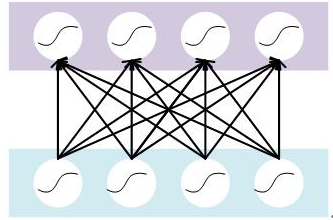
\includegraphics[width=.7\linewidth]{fig_DL/batchnormalization1.png}
     			\caption{Before using Batch normalization}\label{Fig:batchnormalization1}
  		 \end{minipage}\hfill
   		\begin {minipage}{0.48\textwidth}
     			\centering
     			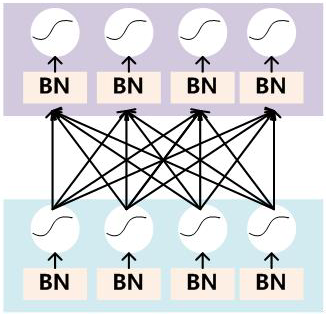
\includegraphics[width=.7\linewidth]{fig_DL/batchnormalization2.png}
     			\caption{After using Batch normalization}\label{Fig:batchnormalization2}
   		\end{minipage}
	\end{figure} \par
	Before adding the batch normalization, the equation for the upper layer is:
	\begin{equation}
		\bm{h}=g(\bm{W^Tu+b})
	\end{equation}
	where $\bm{W}$ and $\bm{b}$ are parameters and $\bm{u}$ is the output of the lower layer.\par
	After the batch normalization is added, the equation for the upper layer becomes:
	\begin{equation}
		\bm{h}=g(\bm{\bm{\hat{x}}})
	\end{equation}
	where, 
	\begin{equation}
		\bm{\hat{x}}=\frac{\bm{x}-E[\bm{x}]}{\sqrt{Var[\bm{x}]}}
	\end{equation}
	and $\bm{x}=\bm{W^Tu+b}$. \par
	In the original paper\citep{ioffe2015batch}, they added a scale and shift to the normalized value, to prevent the change of what the layer can represent. 
	\begin{equation}
		\bm{y}=\gamma \bm{\hat{x}}+\beta
	\end{equation} \par
	For the application of batch normalization on RNN, reference this paper\citep{cooijmans2016recurrent}, the scale parameter should be set to small, like 0.1. \par
%=======================================
\section{Chapter 10 Sequence modeling: Recurrent and recursive nets}
\subsection{Recurrent Neural Networks (\$10.2)}
For equation (10.18):
\begin{equation}\begin{split}
	L^{(t)} =& -\sum_{i}y_{i}^{(t)}log[\hat{y}_{i}^{(t)}] \\
	\overset{(10.11)}{=}& -\sum_{i}y_{i}^{(t)}log[softmax(\mathbf{o^{(t)}})_{i}] \\
	=& -\sum_{i}y_{i}^{(t)}log[\frac{exp(\mathbf{o^{(t)}}_{i})}{\sum_{k}exp(\mathbf{o^{(t)}_{k}})}]
\end{split}\end{equation}
\begin{equation}\begin{split}
	\frac{\partial L^{(t)}}{\partial o_i^{(t)}}
	&=-\frac{\partial}{\partial o_i^{(t)}} \sum_{i}y_{i}^{(t)} \{o_i^{(t)}-log[\sum_{k}exp(\mathbf{o^{(t)}_{k}})] \}\\
	&=-\frac{\partial}{\partial o_i^{(t)}} \{\sum_{i}y_{i}^{(t)} o_i^{(t)}-\sum_{i}y_{i}^{(t)} log[\sum_{k}exp(\mathbf{o^{(t)}_{k}})] \}\\
	&=-y_{i}^{(t)} + [\sum_{i}y_{i}^{(t)}] \cdot [\frac{exp(\mathbf{o^{(t)}}_{i})}{\sum_{k}exp(\mathbf{o^{(t)}_{k}})}]\\
	&=-y_{i}^{(t)} + \hat{y}_{i}^{(t)} = \hat{y}_{i}^{(t)} - y_{i}^{(t)} =  \hat{y}_{i}^{(t)} - \mathbf{1}_{y_{i}^{(t)}=1}
\end{split}\end{equation} \par
For equation (10.19): \par
Scalar L, matrix V, vectors \textbf{o} and \textbf{h} has the realation:  
\begin{equation}\begin{split}
	\mathbf{o}=\mathbf{Vh} \Leftrightarrow
	\begin{bmatrix}
		o_1\\ o_2\\ \vdots\\ o_m\\
	\end{bmatrix}=
	\begin{bmatrix}
		V_{11} & V_{12} & \cdots & V_{1n}\\
		V_{21} & V_{22} & \cdots & V_{2n}\\
		\vdots & \vdots & \ddots & \vdots\\
		V_{m1} & V_{m2} & \cdots & V_{mn}\\
	\end{bmatrix}
	\begin{bmatrix}
		h_1\\ h_2\\ \vdots\\ h_n\\
	\end{bmatrix};
\end{split}\end{equation}
\begin{equation}\begin{split}
\nabla_{\mathbf{h}} L &= 
\begin{bmatrix}
\frac{\partial L}{\partial h_1},
\ \ \frac{\partial L}{\partial h_2},
\ \ \cdots
\ \ \frac{\partial L}{\partial h_n}\\
\end{bmatrix} \\&= 
\begin{bmatrix}
\sum_{i=1}^{m} \frac{\partial L}{\partial o_i}\frac{\partial o_i}{\partial h_1},
\ \ \sum_{i=1}^{m}  \frac{\partial L}{\partial o_i}\frac{\partial o_i}{\partial h_2},
\ \ \cdots
\ \ \sum_{i=1}^{m}  \frac{\partial L}{\partial o_i}\frac{\partial o_i}{\partial h_n}\\
\end{bmatrix} \\&=
\begin{bmatrix}
	\begin{bmatrix}
	\frac{\partial L}{\partial o_1},
	\ \ \frac{\partial L}{\partial o_2},
	\ \ \cdots
	\ \ \frac{\partial L}{\partial o_m}\\
	\end{bmatrix}
	\begin{bmatrix}
	\frac{\partial o_1}{\partial h_1}\\
	\frac{\partial o_2}{\partial h_1}\\
	\vdots\\
	\frac{\partial o_m}{\partial h_1}\\
	\end{bmatrix},
	\begin{bmatrix}
	\frac{\partial L}{\partial o_1},
	\ \ \frac{\partial L}{\partial o_2},
	\ \ \cdots
	\ \ \frac{\partial L}{\partial o_m}\\
	\end{bmatrix}
	\begin{bmatrix}
	\frac{\partial o_1}{\partial h_2}\\
	\frac{\partial o_2}{\partial h_2}\\
	\vdots\\
	\frac{\partial o_m}{\partial h_2}\\
	\end{bmatrix},
\ \ \cdots,
	\begin{bmatrix}
	\frac{\partial L}{\partial o_1},
	\ \ \frac{\partial L}{\partial o_2},
	\ \ \cdots
	\ \ \frac{\partial L}{\partial o_m}\\
	\end{bmatrix}
	\begin{bmatrix}
	\frac{\partial o_1}{\partial h_n}\\
	\frac{\partial o_2}{\partial h_n}\\
	\vdots\\
	\frac{\partial o_m}{\partial h_n}\\
	\end{bmatrix}
\end{bmatrix} \\&= 
\begin{bmatrix}
\frac{\partial L}{\partial o_1},
\ \ \frac{\partial L}{\partial o_2},
\ \ \cdots
\ \ \frac{\partial L}{\partial o_m}\\
\end{bmatrix}
\begin{bmatrix}
\frac{\partial o_{1}}{\partial h_1} & \frac{\partial o_{1}}{\partial h_2} & \cdots & \frac{\partial o_{1}}{\partial h_n}\\
\frac{\partial o_{2}}{\partial h_1} & \frac{\partial o_{2}}{\partial h_2} & \cdots & \frac{\partial o_{2}}{\partial h_n}\\
\vdots & \vdots & \ddots & \vdots\\
\frac{\partial o_{m}}{\partial h_1} & \frac{\partial o_{m}}{\partial h_2} & \cdots & \frac{\partial o_{m}}{\partial h_n}\\
\end{bmatrix} \\&= 
\nabla_{\mathbf{o}} L \ \mathbf{V}
\end{split}\end{equation}
\subsection{Bidirectional RNNs (\$10.3)}
	Used for handwriting recognition, speech recognition and bioinformatics.
\subsection{Encoder-Decoder Sequence-to-Sequence Architectures (\$10.4)}
	Used for Machine Translation.
\subsection{Deep Recurrent Networks (\$10.5)}
\subsection{Recursive Neural Networks (\$10.6)}
%=======================================
\section{Chapter 11 Practical Methodology}
Practical design process:
\begin{enumerate}
	\item Determine error metric and target value;
	\item Establish a Baseline Model;
	\item Determine bottlenecks in performance;
	\item Repeatedly make incremental changes: gathering new data, adjusting hyperparameters, or changing algorithms;
\end{enumerate}
\subsection{Basic recipe for machine learning}
\begin{enumerate}
	\item High bias(training data performance):\par
	\begin{enumerate}
		\item Bigger network
		\item Train longer
		\item Change NN architecture 
	\end{enumerate}
	\item High variance(data set performance):\par
	\begin{enumerate}
		\item More data
		\item Regularization
		\item Change NN architecture 
	\end{enumerate}	
\end{enumerate}
\subsection{Determining Whether to Gather More Data (\$11.3)}
\begin{enumerate}
	\item Determine whether the performance on the training set is acceptable; \par
	If performance on the training set is poor:
	\item Increase the size of the model: add more layers; add more hidden unites to each layer; turning 
	the learning rate etc. \par
	If still not work well: data needed to be cleaned or gathered; \par
	Else:
	\item Measure performance on test set; \par
	If performance good, done!\par
	Else if test set performance is much worse than training set performance:
	\item Gather data;\par
	If not easy to gather data:
	\item Reduce the size of the model; Improve regularization(adjust weight decay coefficients or add dropout); \par
	If test set performance is still unacceptable:
	\item Gather data;
\end{enumerate}
%=======================================
\section{Chapter 12 Applications}
\subsection{Attention Model (\$12.4.5.1)}
	Attention model was first applied in NLP by Bahdanau et al.\citep{bahdanau2014neural} on \textbf{Neural Machine Translation}.\par
	And later Rush et al.\citep{rush2015neural} implemented \textbf{sentence-level summarization} task using it. \par
	Wang et al.\citep{wang2016inner} experimented on \textbf{answer selection} and showed the advantage of inner attention compared with traditional attention methods. \par
	Yin et al.\citep{yin2016simple} tackled \textbf{simple question answering} by an attentive convolutional neural network. \par
%=======================================
\section{Chapter 13 Linear Factor Models}
First, we sample the hidden variables $\bm{h}$:
\begin{equation}
	\bm{h} \sim p(\bm{h})
\end{equation} \par
\textbf{Linear Factor Model} is defined by the use of a stochastic linear decoder function that generates $\bm{x}$ by adding noise to a linear transformation of $\bm{h}$:
\begin{equation}
	\bm{x} = \bm{Wh}+\bm{b}+noise
\end{equation} \par
\subsection{Factor Analysis}
	\textbf{Factor Analysis} assume the hidden variable is the unit variance Gaussian:
	\begin{equation}
		\bm{h} \sim \mathcal{N}(\bm{h;0,I})
	\end{equation} \par
	And assume the \textbf{noise} is drawn from a diagonal covariance Gaussian distribution:
	\begin{equation}
		\bm{x} = \bm{Wh}+\bm{b}+\bm{z}
	\end{equation} \par	
	where $\bm{z} \sim \mathcal{N}(\bm{z;0,\psi})$, with covariance matrix $\bm{\psi} = diag(\bm{\sigma^2})$, $\bm{\sigma^2}=[\sigma_1^2, \sigma_2^2,...,\sigma_n^2]^T$ a vector of per-variable variances. Equivalently, \par
	\begin{equation}
		\bm{x} \sim \mathcal{N}(\bm{x;b,WW^T+\psi})
	\end{equation} \par
	The observable variables $x_i$ are assumed to be \textbf{conditionally independent}, given $\bm{h}$.
\subsection{Probabilistic PCA}
	\textbf{Probabilistic PCA} is based on Factor Analysis with an extra assume of $\sigma_i^2$ equal to each other:
	\begin{equation}
		\bm{x} = \bm{Wh}+\bm{b}+\bm{z}
	\end{equation} \par
	where $\bm{z} \sim \mathcal{N}(\bm{z;0,}\sigma ^2\bm{I})$. Equivalently, \par
	\begin{equation}
		\bm{x} \sim \mathcal{N}(\bm{x;b,WW^T+\sigma^2 \bm{I}})
	\end{equation} \par
\subsection{Sparse Coding}
	\textbf{Sparse Coding} choose the distribution of $\bm{h}$ to be one with sharp peak near 0, like factorized Laplace:
	\begin{equation}
		p(h_i)=Laplace(h_i;0,\frac{2}{\lambda})=\frac{\lambda}{4}e^{-\frac{\lambda |h_i|}{2}}
	\end{equation} \par
	And assume the linear factors have Gaussian noise with isotropic precision $\beta$:
	\begin{equation}
		\bm{x} = \bm{Wh}+\bm{b}+ \bm{z}
	\end{equation} \par
	where $\bm{z} \sim \mathcal{N}(\bm{z;0,} \frac{1}{\beta}\bm{I})$. Now because $\bm{h}$ is not Gaussian as factor analysis, so $\bm{x}$ could not explicitly expressed in Gaussian form like before, thus, equivalently,
	\begin{equation}
		p(\bm{x}|\bm{h}) = \mathcal{N}(\bm{x;Wh+b,}\frac{1}{\beta} \bm{I})
	\end{equation} \par	 
\subsection{Slow Feature Analysis}
	Slow feature analysis is to regularize our model to learn features that change slowly over time, by adding a term to the cost function of the form:
	\begin{equation}
		\lambda \sum_t L(f(\bm{x}^{(t+1)}),f(\bm{x}^{(t)}))
	\end{equation}
	where t is the index into a time sequence of examples, L is a loss function measuring the distance between $f(\bm{x}^{(t)})$ and $f(\bm{x}^{(t+1)})$.
%=======================================
\section{Chapter 14 Autoencoders}
Learning process of autoencoders is minimizing a loss function:
\begin{equation}
	L(\bm{x},g(f(\bm{x})))
\end{equation}
where L is a loss function penalizing $g(f(\bm{x}))$ for being dissimilar from $\bm{x}$, such as the mean square error.
\subsection{Undercomplete Autoencoders}
	One way to obtain useful features from the autoencoder is to contain $\bm{h}$ to have a smaller dimension that $\bm{x}$. That's called \textbf{undercomplete autoencoder}.
\subsection{Regularized Autoencoders}
\subsubsection{Sparse Autoencoders}
	A sparse autoencoder is simply an autoencoder whose training criterion involves a sparsity penalty $\Omega(\bm{h})$ on the code layer $\bm{h}$:
	\begin{equation}
		L(\bm{x},g(f(\bm{x})))+\Omega(\bm{h})
	\end{equation}
	where $g(\bm{h})$ is the decoder output, and typically we have $\bm{h}=f(\bm{x})$, the encoder output. \par
	For example, $\Omega(\bm{h})$ could be:
	\begin{equation}
		\Omega(\bm{h})=\lambda \sum_i |h_i|
	\end{equation}	
\subsubsection{Denoising Autoencoders}
	A denoising autoencoder (DAE) minimizes:
	\begin{equation}
		L(\bm{x},g(f(\bm{\tilde{x}})))
	\end{equation}	
	where $\bm{\tilde{x}}$ is a copy of $\bm{x}$ that has been corrupted by some form of noise.
\subsubsection{Contractive Autoencoders}
	\begin{equation}
		L(\bm{x},g(f(\bm{x})))+\Omega(\bm{h,x})
	\end{equation}
	where,
	\begin{equation}
		\Omega(\bm{h,x})=\lambda \sum_i  ||{\nabla_{\bm{x}} h_i}||^2
	\end{equation}
\subsection{Predictive Sparse Decomposition}
Predictive sparse decomposition (PSD) is a model that is a hybrid of sparse coding and parametric autoencoders. Training proceeds by minimizing:
	\begin{equation}
		||\bm{x}-g(\bm{x})||^2 + \lambda |\bm{h}|_1 + \gamma ||\bm{x}-f(\bm{x})||^2
	\end{equation}
\subsection{Applications of Autoencoders}
\begin{enumerate}
	\item Dimensionality reduction
	\item Information retrieval
\end{enumerate}
%=======================================
\section{Chapter 17 Monte Carlo Methods}
\subsection{Importance Sampling}
\subsection{Markov Chain Monte Carlo Methods}
\subsection{Gibbs Sampling}
%=======================================
\section{Chapter 18 Confronting the Partition Function}
We must normalize the probability distribution in probabilistic models by dividing a partition function $Z(\bm{\theta})$, while it is intractable for many models.
\subsection{Estimate only the gradient of the log partition function}
\subsubsection{Stochastic Maximum Likelihood(SML)}
\subsubsection{Contrastive Divergence(CD)}
\subsection{Training the model without computing the partition function}
\subsubsection{Pseudolikelihood}
\subsubsection{Score Matching and Ratio Matching}
\subsection{Noise-Contrastive Estimation(NCE)}
\subsection{Estimating the Partition Function directly}
%=======================================
\section{Chapter 19 Approximate Inference}
The challenge of inference usually refers to the difficulty of computing $p(\bm{h}|\bm{v})$.\par
\subsection{Inference as Optimization }
\subsection{Expectation Maximization(EM)}
\subsection{MAP Inference and Sparse Coding}
\subsection{Variational Inference and Learning}
\subsection{Learned Approximate Inference} 
%=======================================
\section{Chapter 20 Deep Generative Models}
\subsection{Generative Models and Discriminative Models\citep{ng2002discriminative}}
	For input $\bm{x}$ and output $\bm{y}$, \par
	Generative Models: $p(\bm{x,y})$; \par
	Discriminative Models: $p(\bm{y|x})$. \par
	\par
	\begin{figure}[H]
		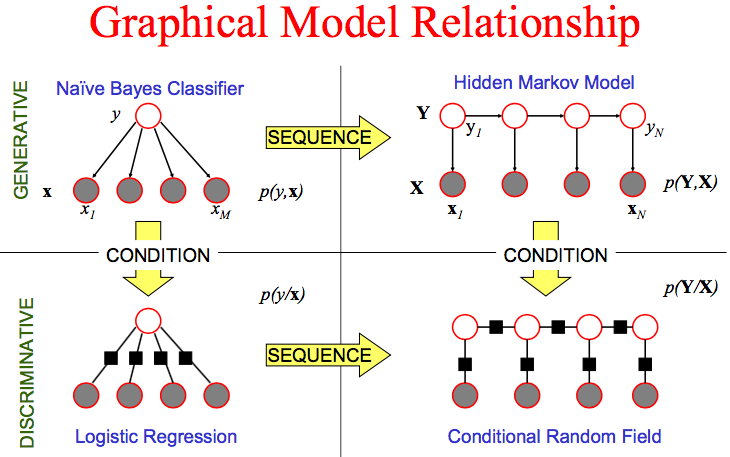
\includegraphics[width=\linewidth]{fig_DL/generative_discriminative_models.png}
		\caption{Generative and Discriminative Models}
		\label{fig:generative_discriminative_models}
	\end{figure}
\subsection{RBM, DBN and DBM (\$20.1 $\sim$ \$20.8)}
\subsection{Directed Generative Nets (\$20.10)}
	Until roughly 2013, the deep learning community have been overshadowed by undirected models such as RBM.
\subsubsection{Sigmoid Belief Networks}
	Sigmoid Belief Networks is a universal approximator of  probability distributions over the visible units.\par
	Inference over the hidden units given the visible units is intracatable.\par
\subsubsection{Differentiable Generator Networks}
\subsubsection{Variational Autoencoders(VAE)}
	A VAE consists of a encoder $q(\bm{z}|\bm{x})$, a decoder $p_{model}(\bm{x}|\bm{z})$ and a loss function $\mathcal{L}(q)$ to minimize: \par
	\begin{equation}
		\mathcal{L}(q) = \sum^N_{i=1} l_i=\sum^N_{i=1}-E_{z \sim q(z|x_i)}[log \ p_{model}(x_i|z)] + D_{KL}(q(z|x_i)||p(z))
	\end{equation}
where $x_i$ is a single datapoint. \par
	The first term is the \textbf{reconstruction loss} of the i-th datapoint. The expectation is taken with respect to the \textbf{encoder's distribution over the representations}. This term encourages the decoder to learn to reconstruct the data, if the decoder's output does not reconstruct the data well, it will incur a large cost in this loss function. \par
	The second term is a regularizer. It's the KL divergence between the encoder's distribution $q(z|x_i)$ and $p(z)$. It is one measure of how close q is to p. In VAE, p is specified as a Gaussian distribution. If the encoder outputs that are different than those from a Gaussian distribution, it will receive a penalty in the loss function. This regularizer term means to "keep the representations z of each datapoint sufficiently diverse". If we didn't include the regularizer, the encoder could learn to cheat and give each datapoint a representation in a different region of Euclidean space. This is bad, because for example in the case of hand writing of number 2 of two different people, could end up with very different representations. We need the representation space of z to be meaningful, so we penalize this behavior. This has the effect of keeping similar numbers' representations close together. \par
	We train the VAE using gradient descent to minimize the loss with respect to the parameters of the encoder and decoder. \par
	\paragraph{The probability model perspective} \par
	A VAE contains a specific probability model of data x and latent variables z. And we have $p(x,z)=p(x|z)p(z)$. The generative process can be written as: \par
	For each datapoint i:
	\begin{enumerate}
		\item Draw latent variables from the prior: $z_i \sim p(z)$
		\item Draw datapoint from the likelihood: $x_i \sim p(x|z)$
	\end{enumerate} \par
	Now, the goal is to infer good values of the latent variables given observed data, or to calculate the posterior $p{z|x}$:
	\begin{equation}
		p(z|x)=\frac{p(x|z)p(z)}{p(x)}
	\end{equation} \par
	The denominator $p(x)$ is called the evidence, could be calculated by marginalizing out the latent variables:$p(x)=\int p(x|z)p(z)dz$. And it is difficult to calculate, so need to approximate(ref. Chapter 19). \par
	Variation inference approximates the posterior with distribution $q(z|x)$. Then follow the derivatives in page 624, we get the same loss function. And use EM for learning. \par
\subsubsection{Generative Adversarial Networks(GANs)\citep{goodfellow2014generative}}
	A GAN consists of a generator $g(\bm{z;\theta}^{(g)})$, a discriminator $d(\bm{x;\theta}^{(d)})$. \par
	We first define a prior on input noise variables $p_z(z)$, then generate data $\bm{x}$ using $g(\bm{z;\theta}^{(g)})$, which is a differentiable function represented by a multilayer perceptron with the parameter $\bm{\theta}^{(g)}$. \par
	Then we use $d(\bm{x;\theta}^{(d)})$ on the generated data $\bm{x}$ to output a single scalar, which represents the probability that $\bm{x}$ came from the data rather than the prior $p_z(z)$. \par
	We train $d(\bm{x;\theta}^{(d)})$ to maximize the probability of assigning the correct label to both training examples and samples from $g(\bm{z;\theta}^{(g)})$. \par
	Simultaneously, we train $g(\bm{z;\theta}^{(g)})$ to minimize $log(1-d(g(\bm{z})))$. \par
	In other words, d and g play the following two-player minimax game with value function v:
	\begin{equation}
		\mathop{min}_{g} \mathop{max}_{d} v(\bm{\theta}^{(g)}, \bm{\theta}^{(d)}) 
		= \mathop{min}_{g} \mathop{max}_{d}
		\{ \mathbb{E}_{\bm{x} \sim p_{data}} [log \ d(\bm{x})] + 
		\mathbb{E}_{\bm{z} \sim p_{z}} [log \ (1-d(g(\bm{z})))] \}
	\end{equation} \par
	\begin{algorithm}
	\caption{Minibatch stochastic gradient descent training of generative adversarial nets. The number of steps to apply to the discriminator, k, is a hyperparameter. We used k = 1, the least expensive option, in our experiments.}\label{euclid}
	\begin{algorithmic}[]	
	\For{number of training iterations}
		\For{k steps}
            		\begin{itemize}
			\item Sample minibatch of m noise samples ${z^{(1)}, . . . , z^{(m)}}$ from noise prior $p_g(\bm{z})$.
			\item Sample minibatch of m noise samples ${x^{(1)}, . . . , x^{(m)}}$ from data generating distribution $p_{data}(\bm{x})$.
			\item Update the discriminator by ascending its stochastic gradient:
			\begin{align*}
				\nabla_{\theta_d}\frac{1}{m}\sum_{i=1}^m [log \ d(\bm{x}^{(i)})+ log \ (1-d(g(\bm{z}^{(i)})))]
			\end{align*}
			\end{itemize}
		\EndFor
		\begin{itemize}
			\item Sample minibatch of m noise samples ${z^{(1)}, . . . , z^{(m)}}$ from noise prior $p_g(\bm{z})$.
			\item Update the discriminator by ascending its stochastic gradient:
			\begin{align*}
				\nabla_{\theta_g}\frac{1}{m}\sum_{i=1}^m log \ (1-d(g(\bm{z}^{(i)})))
			\end{align*}
			\end{itemize}
        \EndFor \par
        The gradient-based updates can use any standard gradient-based learning rule. We used momentum in our experiments.
	\end{algorithmic}
	\end{algorithm}
\subsubsection{Generative Moment Matching Networks}
\subsubsection{Convolution Generative Networks}
\subsubsection{Auto-Regressive Networks}
	Auto-regressive networks are directed probabilistic models with no latent random variables. Such models have been called \textbf{fully-visible Bayes networks}(FVBNs).\par
\subsubsection{Linear Auto-Regressive Networks}
	The simplest form of auto-regressive networks has no hidden units and no sharing of parameters or features. Each $P(x_i|x_{i-1},...,x_1)$ is parametrized as a linear model. \par
	Linear auto-regressive networks are essentially the generalization of linear classification methods to generative modeling. \par
\subsubsection{Neural Auto-Regressive Netvorks}
	With the same graphical model as linear auto-regression networks but the different parametrization of the conditional distributions $P(x_i|x_{i-1},...,x_1)$, which now is parametrized by a neural network. \par
\subsubsection{Neural Auto-Regressive Density Estimator(NADE)}
	NADE is the same as the original neural auto-regressive networks, but introduces an additional parameter sharing scheme. The parameters of the hidden unites of different groups are shared.\par
\subsection{Autoencoders (\$20.11 $\sim$ \$20.12)}
\subsection{Other Generation Schemes (\$20.13)}
\subsubsection{Diffusion Inversion}
\subsubsection{Approximate Bayesian Computation(ABC)}
\subsection{Evaluating Generative Models (\$20.14)}
%=======================================
\section{NLP - Language Model}
Finite set of all the words W; Ex: W = \{the, a, man, bag, dogs, ...\}. \par
Set of all the REAL sequences of words L; Ex: L = \{the, a, the fan, the fan saw Beckham, the fan saw saw, ...\}.\par
We have a sample set of sequences of words S.\par
Now we need to learn the REAL probability distribution $p$, where:
\[
\sum_{x \in L} p(x) = 1
\]\par
Old method to calculate $p_{L}$:
\begin{enumerate}
	\item Assuming that $|S| = N$;
	\item c(x) is the number of appearances of x in T;
	\item Then, $p(x)=\frac{c(x)}{N} $.
\end{enumerate}
Problem of this method: If a sequences of words $x \in S$ does not in sample set T, so $p(x)=0$;
But if it exists in S, then $p(x) \neq 0$.
\subsection{Markov Processes and N-gram}
To solve this problem, we assume a random variables $X_1, X_2, X_3, ..., X_n$, for each of them can take any value in the word set W. \par
The word sequence $x \in T$ can be represented by the words: $x = \{x_1, x_2, x_3, ..., x_n\}$, where $x_i \in W$;\par
First-order Markov Processes(the probability of the word is depend only on ONE word before):
\begin{equation}\begin{split}
&P(X_1=x_1, X_2=x_2, ..., X_n=x_n)\\ 
=&P(X_1=x_1)\prod_{i=2}^{n}P(X_i=x_i|X_1=x_1, ..., X_{i-1}=x_{i-1})\\ 
=&P(X_1=x_1)\prod_{i=2}^{n}P(X_i=x_i|X_{i-1}=x_{i-1}) 
\end{split}\end{equation}
Second-order Markov Processes(the probability of the word is depend only on TWO words before):
\begin{equation}
	P(X_1=x_1, X_2=x_2, ..., X_n=x_n)=\prod_{i=1}^{n}P(X_i=x_i|X_{i-2}=x_{i-2}, X_{i-1}=x_{i-1}) 
\end{equation}
where $x_0=x_1=START$.\par
Trigram Language Model:\par
For every $x = \{x_1, x_2, x_3, ..., x_n\} \in T$, we have:
\begin{equation}
p(\{x_1, x_2, ..., x_n\})=\prod_{i=1}^{n}q(x_i|\{x_{i-2}, x_{i-1}\}) 
\end{equation}
where $x_0=x_1=START$, and $q(x_i|\{x_{i-2}, x_{i-1}\})=\frac{c(\{x_i, x_{i-2}, x_{i-1}\})}{c(\{x_{i-2}, x_{i-1}\})}$ \par
Problem of this method: for example, $q(laughs|\{the, dog\})=\frac{c(\{the, dog, laughs\})}{c(\{the, dog\})}$; if there is no phase "the dog laughs" in the sample set, then $q(laughs|\{the, dog\})=0$, that is not the case; And if there is no phase "the dog", then $c(\{the, dog\})=0$, it will cause a problem of division.
\subsection{Evaluation of Language Models: Perplexity}
According to Maximum Likelihood Estimation, a good model should assign probability: $\prod_{i=1}^{N}p(s_i)$ where $s_i \in S$ as as high as possible.
\begin{equation}
Perplexity=2^{-\frac{1}{N}\sum_{i=1}^{N}log p(s_i)}
\end{equation}
So a better model should have a lower Perplexity.
%=======================================
\section{Course 2 Practical aspects of Deep Learning} 
\subsection{Practice Questions - Week 1}
\begin{enumerate}
	\item If you have 10,000,000 examples, how would you split the train/dev/test set?
	\begin{enumerate}
		\item 33\% train . 33\% dev . 33\% test
		\item 98\% train . 1\% dev . 1\% test
		\item 60\% train . 20\% dev . 20\% test
	\end{enumerate}\par
	Answer: b.
	\item The dev and test set should:
	\begin{enumerate}
		\item Come from the same distribution
		\item Come from different distributions
		\item Be identical to each other (same (x, y) pairs)
		\item Have the same number of example
	\end{enumerate}\par
	Answer: a.
	\item If your Neural Network model seems to have high variance, what of the following would be promising things to try?
	\begin{enumerate}
		\item Increase the number of units in each hidden layer
		\item Make the Neural Network deeper
		\item Get more test data
		\item Add regularization
		\item Get more training data
	\end{enumerate}\par
	Answer: d, e. If the question is to have high bias, the answer should be: a, b.
	\item You are working on an automated check-out kiosk for a supermarket, and are building a classifier for apples, bananas and oranges. Suppose your classifier obtains a training set error of 0.5\%, and a dev set error of 7\%. Which of the following are promising things to try to improve your classifier? (Check all that apply.)
	\begin{enumerate}
		\item Increase the regularization parameter lambda
		\item Decrease the regularization parameter lambda
		\item Get more training data
		\item Use a bigger neural network
	\end{enumerate}\par
	Answer: a, c.
	\item What is weight decay?
	\begin{enumerate}
		\item A technique to avoid vanishing gradient by imposing a ceiling on the values of the weights.
		\item A regularization technique (such as L2 regularization) that results in gradient descent shrinking the weights on every iteration.
Correct 
		\item The process of gradually decreasing the learning rate during training.
		\item Gradual corruption of the weights in the neural network if it is trained on noisy data.
	\end{enumerate}\par
	Answer: b.
	\item What happens when you increase the regularization hyperparameter lambda?
	\begin{enumerate}
		\item Weights are pushed toward becoming smaller (closer to 0)
		\item Weights are pushed toward becoming bigger (further from 0)
		\item Doubling lambda should roughly result in doubling the weights
		\item Gradient descent taking bigger steps with each iteration (proportional to lambda)
	\end{enumerate}\par
	Answer: a.
	\item With the inverted dropout technique, at test time:
	\begin{enumerate}
		\item You apply dropout (randomly eliminating units) but keep the 1/keep\_prob factor in the calculations used in training.
		\item You do not apply dropout (do not randomly eliminate units), but keep the 1/keep\_prob factor in the calculations used in training.
		\item You do not apply dropout (do not randomly eliminate units) and do not keep the 1/keep\_prob factor in the calculations used in training
		\item You apply dropout (randomly eliminating units) and do not keep the 1/keep\_prob factor in the calculations used in training
	\end{enumerate}\par
	Answer: c.
	\item Increasing the parameter keep\_prob from (say) 0.5 to 0.6 will likely cause the following: (Check the two that apply)
	\begin{enumerate}
		\item Increasing the regularization effect
		\item Reducing the regularization effect
		\item Causing the neural network to end up with a higher training set error
		\item Causing the neural network to end up with a lower training set error
	\end{enumerate}\par
	Answer: b, d.
	\item Which of these techniques are useful for reducing variance (reducing overfitting)? (Check all that apply.)
	\begin{enumerate}
		\item Xavier initialization
		\item Dropout
		\item Vanishing gradient
		\item Gradient Checking
		\item L2 regularization
		\item Exploding gradient
		\item Data augmentation
	\end{enumerate}\par
	Answer: b, e, g.
	\item Why do we normalize the inputs x?
	\begin{enumerate}
		\item It makes the cost function faster to optimize
		\item It makes it easier to visualize the data
		\item Normalization is another word for regularization--It helps to reduce variance
		\item It makes the parameter initialization faster
	\end{enumerate}\par
	Answer: a.	
\end{enumerate}
\section{Course 3 Structuring Machine Learning Project} 
\subsection{Bird recognition in the city of Peacetopia (case study)}
You are a famous researcher in the City of Peacetopia. The people of Peacetopia have a common characteristic: they are afraid of birds. To save them, you have to build an algorithm that will detect any bird flying over Peacetopia and alert the population. \par
The City Council gives you a dataset of 10,000,000 images of the sky above Peacetopia, taken from the city's security cameras. They are labelled:
\begin{itemize}
	\item y = 0: There is no bird on the image
	\item y = 1: There is a bird on the image
\end{itemize}
Your goal is to build an algorithm able to classify new images taken by security cameras from Peacetopia.\par
There are a lot of decisions to make:
\begin{itemize}
	\item What is the evaluation metric?
	\item How do you structure your data into train/dev/test sets?
\end{itemize}
\begin{enumerate}
	\item Metric of success \par
	The City Council tells you the following that they want an algorithm that
	\begin{enumerate}
		\item Has high accuracy
		\item Runs quickly and takes only a short time to classify a new image.
		\item Can fit in a small amount of memory, so that it can run in a small processor that the city will attach to many different security cameras.
	\end{enumerate}
	Note: Having three evaluation metrics makes it harder for you to quickly choose between two different algorithms, and will slow down the speed with which your team can iterate. True/False? \par
	Answer: True.
	\item After further discussions, the city narrows down its criteria to: 
	\begin{itemize}
		\item "We need an algorithm that can let us know a bird is flying over Peacetopia as accurately as possible."
		\item "We want the trained model to take no more than 10sec to classify a new image."
		\item "We want the model to fit in 10MB of memory."
	\end{itemize}
	If you had the three following models, which one would you choose?
	\begin{table}[h!]
  		\centering
  		\begin{tabular}{c|c|c|c}
   			& Test Accuracy & Runtime & Memory size\\
   			\hline
    			1 & 97\% & 1 sec & 3MB\\
			2 & 99\% & 13 sec & 9MB\\
			3 & 97\% & 3 sec & 2MB\\
			4 & 98\% & 9 sec & 9MB\\
  		\end{tabular}
	\end{table} \par
	Answer: 4.
	\item Based on the city's requests, which of the following would you say is true?
		\begin{enumerate}
		\item Accuracy is an optimizing metric; running time and memory size are a satisficing metrics.
		\item Accuracy is a satisficing metric; running time and memory size are an optimizing metric.
		\item Accuracy, running time and memory size are all optimizing metrics because you want to do well on all three.
		\item Accuracy, running time and memory size are all satisficing metrics because you have to do sufficiently well on all three for your system to be acceptable.
		\end{enumerate} \par
	Answer: 1.
	\item Structuring your data \par
	Before implementing your algorithm, you need to split your data into train/dev/test sets. Which of these do you think is the best choice? 
	\begin{table}[h!]
  		\centering
  		\begin{tabular}{c|c|c|c}
   			& Train & Dev & Test \\
   			\hline
    			1 & 6,000,000 & 1,000,000 & 3,000,000\\
			2 & 6,000,000 & 3,000,000 & 1,000,000\\
			3 & 3,333,334 & 3,333,334 & 3,333,334\\
			4 & 9,500,000 & 250,000 & 250,000\\
  		\end{tabular}
	\end{table} \par
	Answer: 4.
	\item After setting up your train/dev/test sets, the City Council comes across another 1,000,000 images, called the "citizens' data". Apparently the citizens of Peacetopia are so scared of birds that they volunteered to take pictures of the sky and label them, thus contributing these additional 1,000,000 images. These images are different from the distribution of images the City Council had originally given you, but you think it could help your algorithm. \par
	You should not add the citizens' data to the \textbf{training set}, because this will cause the training and dev/test set distributions to become different, thus hurting dev and test set performance. True/False? \par
	Answer: False. I should add the citizens' data to the \textbf{training set}. Adding this data to the training set will change the training set distribution. However, it is not a problem to have different training and dev distribution. On the contrary, it would be very problematic to have different dev and test set distributions.
	\item One member of the City Council knows a little about machine learning, and thinks you should add the 1,000,000 citizens? data images to the \textbf{test set}. You object because:
		\begin{enumerate}
		\item The 1,000,000 citizens' data images do not have a consistent x-->y mapping as the rest of the data (similar to the New York City/Detroit housing prices example from lecture).
		\item The test set no longer reflects the distribution of data (security cameras) you most care about.
		\item A bigger test set will slow down the speed of iterating because of the computational expense of evaluating models on the test set.
		\item This would cause the dev and test set distributions to become different. This is a bad idea because you're not aiming where you want to hit.
		\end{enumerate} \par
	Answer: 2,4.
	\item You train a system, and its errors are as follows (error = 100\%-Accuracy):\par
	Training set error: 4.0\%; Dev set error: 4.5\%. \par
	This suggests that one good avenue for improving performance is to train a bigger network so as to drive down the 4.0\% training error. Do you agree? \par
	Answer: No, because there is insufficient information to tell.
	\item You ask a few people to label the dataset so as to find out what is human-level performance. You find the following levels of accuracy: \par
	\begin{table}[h!]
  		\centering
  		\begin{tabular}{c|c}
    			Bird watching expert \#1 & 0.3\% error\\ \hline
			Bird watching expert \#2 & 0.5\% error\\ \hline
			Normal person \#1 (not a bird watching expert) & 1.0\% error\\ \hline
			Normal person \#2 (not a bird watching expert) & 1.2\% error\\
  		\end{tabular}
	\end{table} \par
	If your goal is to have "human-level performance" be a proxy (or estimate) for Bayes error, how would you define "human-level performance"?\par
	Answer: 0.3\% 
	\item A learning algorithm's performance can be better human-level performance but it can never be better than Bayes error.
	\item You find that a team of ornithologists debating and discussing an image gets an even better 0.1\% performance, so you define that as "human-level performance". After working further on your algorithm, you end up with the following:
	\begin{table}[h!]
  		\centering
  		\begin{tabular}{c|c}
    			Human-level performance & 0.1\% \\ \hline
			Training set error & 2.0\% \\ \hline
			Dev set error & 2.1\% \\ 
  		\end{tabular}
	\end{table} \par
	Based on the evidence you have, which two of the following four options seem the most promising to try? (Check two options.)
	\begin{enumerate}
		\item Train a bigger model to try to do better on the training set.
		\item Try decreasing regularization.
		\item Try increasing regularization.
		\item Get a bigger training set to reduce variance.
	\end{enumerate} \par
	Answer: 1,2.
	\item You also evaluate your model on the test set, and find the following:
	\begin{table}[h!]
  		\centering
  		\begin{tabular}{c|c}
    			Human-level performance & 0.1\% \\ \hline
			Training set error & 2.0\% \\ \hline
			Dev set error & 2.1\% \\ \hline
			Test set error & 7.0\% \\ 
  		\end{tabular}
	\end{table} \par
	What does this mean? (Check the two best options.)
	\begin{enumerate}
		\item You have overfit to the dev set.
		\item You should get a bigger test set.
		\item You have underfit to the dev set.
		\item You should try to get a bigger dev set.
	\end{enumerate} \par
	Answer: 1,4.
	\item After working on this project for a year, you finally achieve:
	\begin{table}[h!]
  		\centering
  		\begin{tabular}{c|c}
    			Human-level performance & 0.10\% \\ \hline
			Training set error & 0.05\% \\ \hline
			Dev set error & 0.05\% \\ 
  		\end{tabular}
	\end{table} \par
	What can you conclude? (Check all that apply.)
	\begin{enumerate}
		\item With only 0.09\% further progress to make, you should quickly be able to close the remaining gap to 0\%
		\item If the test set is big enough for the 0,05\% error estimate to be accurate, this implies Bayes error is $\leqslant$ 0.05
		\item It is now harder to measure avoidable bias, thus progress will be slower going forward.
		\item This is a statistical anomaly (or must be the result of statistical noise) since it should not be possible to surpass human-level performance.
	\end{enumerate} \par
	Answer: 2,3.
	\item It turns out Peacetopia has hired one of your competitors to build a system as well. Your system and your competitor both deliver systems with about the same running time and memory size. However, your system has higher accuracy! However, when Peacetopia tries out your and your competitor?s systems, they conclude they actually like your competitor?s system better, because even though you have higher overall accuracy, you have more false negatives (failing to raise an alarm when a bird is in the air). What should you do? \par
	\begin{enumerate}
		\item Look at all the models you?ve developed during the development process and find the one with the lowest false negative error rate.
		\item Ask your team to take into account both accuracy and false negative rate during development.
		\item Rethink the appropriate metric for this task, and ask your team to tune to the new metric.
		\item Pick false negative rate as the new metric, and use this new metric to drive all further development.
	\end{enumerate} \par
	Answer: 3.
	\item You've handily beaten your competitor, and your system is now deployed in Peacetopia and is protecting the citizens from birds! But over the last few months, a new species of bird has been slowly migrating into the area, so the performance of your system slowly degrades because your data is being tested on a new type of data. \par
	You have only 1,000 images of the new species of bird. The city expects a better system from you within the next 3 months. Which of these should you do first?
	\begin{enumerate}
		\item Use the data you have to define a new evaluation metric (using a new dev/test set) taking into account the new species, and use that to drive further progress for your team.
		\item Put the 1,000 images into the training set so as to try to do better on these birds.
		\item Try data augmentation/data synthesis to get more images of the new type of bird.			\item Add the 1,000 images into your dataset and reshuffle into a new train/dev/test split.	\end{enumerate} \par
	Answer: 1.
	\item The City Council thinks that having more Cats in the city would help scare off birds. They are so happy with your work on the Bird detector that they also hire you to build a Cat detector. (Wow Cat detectors are just incredibly useful aren't they.) Because of years of working on Cat detectors, you have such a huge dataset of 100,000,000 cat images that training on this data takes about two weeks. Which of the statements do you agree with? (Check all that agree.)
	\begin{enumerate}
		\item Buying faster computers could speed up your teams' iteration speed and thus your team?s productivity.
		\item Having built a good Bird detector, you should be able to take the same model and hyperparameters and just apply it to the Cat dataset, so there is no need to iterate.
		\item Needing two weeks to train will limit the speed at which you can iterate.
		\item If 100,000,000 examples is enough to build a good enough Cat detector, you might be better of training with just 10,000,000 examples to gain a $\approx$ 10x improvement in how quickly you can run experiments, even if each model performs a bit worse because it's trained on less data.
	\end{enumerate} \par
	Answer: 1, 3, 4.
\end{enumerate}
\subsection{Autonomous driving(case study)}
	You are employed by a startup building self-driving cars. You are in charge of detecting road signs (stop sign, pedestrian crossing sign, construction ahead sign) and traffic signals (red and green lights) in images. The goal is to recognize which of these objects appear in each image. \par
	Your 100,000 labeled images are taken using the front-facing camera of your car. This is also the distribution of data you care most about doing well on. You think you might be able to get a much larger dataset off the internet, that could be helpful for training even if the distribution of internet data is not the same.\par
\begin{enumerate}
	\item You are just getting started on this project. What is the first thing you do? Assume each of the steps below would take about an equal amount of time (a few days).
	\begin{enumerate}
		\item Spend a few days collecting more data using the front-facing camera of your car, to better understand how much data per unit time you can collect.
		\item Spend a few days getting the internet data, so that you understand better what data is available.
		\item Spend a few days training a basic model and see what mistakes it makes.
		\item Spend a few days checking what is human-level performance for these tasks so that you can get an accurate estimate of Bayes error.
	\end{enumerate} \par
	Answer: 3. As discussed in lecture, applied ML is a highly iterative process. If you train a basic model and carry out error analysis (see what mistakes it makes) it will help point you in more promising directions.
	\item Your goal is to detect road signs (stop sign, pedestrian crossing sign, construction ahead sign) and traffic signals (red and green lights) in images. The goal is to recognize which of these objects appear in each image. You plan to use a deep neural network with ReLU units in the hidden layers.\par
For the output layer, a softmax activation would be a good choice for the output layer because this is a multi-task learning problem. True/False? \par
	Answer: False. Softmax would be a good choice if one and only one of the possibilities (stop sign, speed bump, pedestrian crossing, green light and red light) was present in each image.
	\item You are carrying out error analysis and counting up what errors the algorithm makes. Which of these datasets do you think you should manually go through and carefully examine, one image at a time?
	\begin{enumerate}
		\item 10,000 randomly chosen images
		\item 500 images on which the algorithm made a mistake
		\item 10,000 images on which the algorithm made a mistake
		\item 500 randomly chosen images
	\end{enumerate} \par
	Answer: 2. Focus on images that the algorithm got wrong. Also, 500 is enough to give you a good initial sense of the error statistics. There?s probably no need to look at 10,000, which will take a long time.
	\item After working on the data for several weeks, your team ends up with the following data:
	\begin{enumerate}
		\item 100,000 labeled images taken using the front-facing camera of your car.
		\item 900,000 labeled images of roads downloaded from the internet.
		\item Each image?s labels precisely indicate the presence of any specific road signs and traffic signals or combinations of them. For example, $y^{(i)} =\begin{bmatrix} 1\\0\\0\\1\\0\end{bmatrix}$ means the image contains a stop sign and a red traffic light.
	\end{enumerate} \par
Because this is a multi-task learning problem, you need to have all your $y^{(i)}$ vectors fully labeled. If one example is equal to  $y^{(i)} =\begin{bmatrix} 0\\?\\1\\1\\?\end{bmatrix}$ then the learning algorithm will not be able to use that example. True/False? \par
	Answer: False. As seen in the lecture on multi-task learning, you can compute the cost such that it is not influenced by the fact that some entries haven't been labeled.
	\item The distribution of data you care about contains images from your car's front-facing camera; which comes from a different distribution than the images you were able to find and download off the internet. How should you split the dataset into train/dev/test sets? \par
	\begin{enumerate}
		\item Choose the training set to be the 900,000 images from the internet along with 20,000 images from your car's front-facing camera. The 80,000 remaining images will be split equally in dev and test sets.
		\item Choose the training set to be the 900,000 images from the internet along with 80,000 images from your car's front-facing camera. The 20,000 remaining images will be split equally in dev and test sets.
		\item Mix all the 100,000 images with the 900,000 images you found online. Shuffle everything. Split the 1,000,000 images dataset into 980,000 for the training set, 10,000 for the dev set and 10,000 for the test set.
		\item Mix all the 100,000 images with the 900,000 images you found online. Shuffle everything. Split the 1,000,000 images dataset into 600,000 for the training set, 200,000 for the dev set and 200,000 for the test set.
	\end{enumerate} \par
	Answer: 2. It is important that your dev and test set have the closest possible distribution to ?real?-data. It is also important for the training set to contain enough ?real?-data to avoid having a data-mismatch problem.
	\item Assume you've finally chosen the following split between of the data:
	\begin{table}[h!]
  		\centering
  		\begin{tabular}{c|c|c}
   			Dataset & Contains & Error of the algorithm\\
   			\hline
    			Training & \begin{tabular}[x]{@{}c@{}}940,000 images randomly picked from (900,000 internet images  \\+ 60,000 car's front-facing camera images)\end{tabular} & 8.8\%\\
			Training-Dev &\begin{tabular}[x]{@{}c@{}}940,000 images randomly picked from (900,000 internet images  \\+ 60,000 car's front-facing camera images)\end{tabular}  & 9.1\%\\
			Dev & 20,000 images from your car's front-facing camera & 14.3\%\\
			Test & 20,000 images from your car's front-facing camera & 14.8\%\\
  		\end{tabular}
	\end{table} \par
	You also know that human-level error on the road sign and traffic signals classification task is around 0.5\%. Which of the following are True? (Check all that apply).
	\begin{enumerate}
		\item You have a large variance problem because your model is not generalizing well to data from the same training distribution but that it has never seen before.
		\item You have a large data-mismatch problem because your model does a lot better on the training-dev set than on the dev set
		\item You have a large avoidable-bias problem because your training error is quite a bit higher than the human-level error.
		\item Your algorithm overfits the dev set because the error of the dev and test sets are very close.
		\item You have a large variance problem because your training error is quite higher than the human-level error.
	\end{enumerate} \par
	Answer: 2, 3.
	\item Based on table from the previous question, a friend thinks that the training data distribution is much easier than the dev/test distribution. What do you think?
	\begin{enumerate}
		\item Your friend is right. (I.e., Bayes error for the training data distribution is probably lower than for the dev/test distribution.)
		\item Your friend is wrong. (I.e., Bayes error for the training data distribution is probably higher than for the dev/test distribution.)
		\item There's insufficient information to tell if your friend is right or wrong.
	\end{enumerate}\par
	Answer: 3. The algorithm does better on the distribution of data it trained on. But you don't know if it's because it trained on that no distribution or if it really is easier. To get a better sense, measure human-level error separately on both distributions.\par
	\item You decide to focus on the dev set and check by hand what are the errors due to. Here is a table summarizing your discoveries: \par
	\begin{table}[H]
  		\centering
  		\begin{tabular}{l|c}
   			Overall dev set error & 14.3\%\\ \hline
    			Errors due to incorrectly labeled data & 4.1\%\\ \hline
    			Errors due to foggy pictures & 8.0\%\\ \hline
    			Errors due to rain drops stuck on your car?s front-facing camera & 2.2\%\\ \hline
			Errors due to other causes & 1.0\% \\
  		\end{tabular}
	\end{table} \par
	In this table, 4.1\%, 8.0\%, etc.are a fraction of the total dev set (not just examples your algorithm mislabeled). I.e. about 8.0/14.3 = 56\% of your errors are due to foggy pictures.\par
	The results from this analysis implies that the team?s highest priority should be to bring more foggy pictures into the training set so as to address the 8.0\% of errors in that category. True/False?
	\begin{enumerate}
		\item True because it is the largest category of errors. As discussed in lecture, we should prioritize the largest category of error to avoid wasting the team?s time.
		\item True because it is greater than the other error categories added together (8.0 > 4.1+2.2+1.0).
		\item False because this would depend on how easy it is to add this data and how much you think your team thinks it'll help.
		\item False because data augmentation (synthesizing foggy images by clean/non-foggy images) is more efficient.
	\end{enumerate} \par
	Answer: 3.	
	\item You can buy a specially designed windshield wiper that help wipe off some of the raindrops on the front-facing camera. Based on the table from the previous question, which of the following statements do you agree with?
	\begin{enumerate}
		\item 2.2\% would be a reasonable estimate of the maximum amount this windshield wiper could improve performance.
		\item 2.2\% would be a reasonable estimate of the minimum amount this windshield wiper could improve performance.
		\item 2.2\% would be a reasonable estimate of how much this windshield wiper will improve performance.
		\item 2.2\% would be a reasonable estimate of how much this windshield wiper could worsen performance in the worst case.
	\end{enumerate}
	Answer: 1. Yes. You will probably not improve performance by more than 2.2\% by solving the raindrops problem. If your dataset was infinitely big, 2.2\% would be a perfect estimate of the improvement you can achieve by purchasing a specially designed windshield wiper that removes the raindrops.
	\item You decide to use data augmentation to address foggy images. You find 1,000 pictures of fog off the internet, and "add" them to clean images to synthesize foggy days, like this: \par
	\begin{figure}[H]
		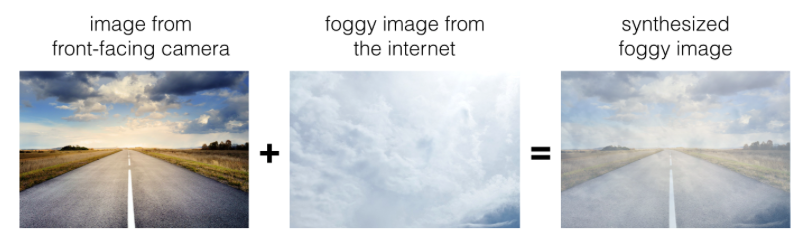
\includegraphics[width=\linewidth]{fig_DL/autodrive.png}
		\caption{}
		\label{fig:}
	\end{figure}
	Which of the following statements do you agree with?
	\begin{enumerate}
		\item There is little risk of overfitting to the 1,000 pictures of fog so long as you are combing it with a much larger ($>>$1,000) of clean/non-foggy images.
		\item Adding synthesized images that look like real foggy pictures taken from the front-facing camera of your car to training dataset won't help the model improve because it will introduce avoidable-bias.
		\item So long as the synthesized fog looks realistic to the human eye, you can be confident that the synthesized data is accurately capturing the distribution of real foggy images, since human vision is very accurate for the problem you're solving.
	\end{enumerate}
	Answer: 3. Yes. If the synthesized images look realistic, then the model will just see them as if you had added useful data to identify road signs and traffic signals in a foggy weather. I will very likely help.
	\item After working further on the problem, you've decided to correct the incorrectly labeled data on the dev set. Which of these statements do you agree with? (Check all that apply).
	\begin{enumerate}
		\item You should also correct the incorrectly labeled data in the test set, so that the dev and test sets continue to come from the same distribution
		\item You should correct incorrectly labeled data in the training set as well so as to avoid your training set now being even more different from your dev set.
		\item You should not correct the incorrectly labeled data in the test set, so that the dev and test sets continue to come from the same distribution
		\item You should not correct incorrectly labeled data in the training set as well so as to avoid your training set now being even more different from your dev set.
	\end{enumerate}
	Answer: 1, 4. Deep learning algorithms are quite robust to having slightly different train and dev distributions.
	\item So far your algorithm only recognizes red and green traffic lights. One of your colleagues in the startup is starting to work on recognizing a yellow traffic light. (Some countries call it an orange light rather than a yellow light; we'll use the US convention of calling it yellow.) Images containing yellow lights are quite rare, and she doesn't have enough data to build a good model. She hopes you can help her out using transfer learning. \par
	What do you tell your colleague?
	\begin{enumerate}
		\item She should try using weights pre-trained on your dataset, and fine-tuning further with the yellow-light dataset.
		\item If she has (say) 10,000 images of yellow lights, randomly sample 10,000 images from your dataset and put your and her data together. This prevents your dataset from ?swamping? the yellow lights dataset.
		\item You cannot help her because the distribution of data you have is different from hers, and is also lacking the yellow label.
		\item Recommend that she try multi-task learning instead of transfer learning using all the data.
	\end{enumerate}
	Answer: 1.You have trained your model on a huge dataset, and she has a small dataset. Although your labels are different, the parameters of your model have been trained to recognize many characteristics of road and traffic images which will be useful for her problem. This is a perfect case for transfer learning, she can start with a model with the same architecture as yours, change what is after the last hidden layer and initialize it with your trained parameters.
	\item Another colleague wants to use microphones placed outside the car to better hear if there?re other vehicles around you. For example, if there is a police vehicle behind you, you would be able to hear their siren. However, they don?t have much to train this audio system. How can you help?
	\begin{enumerate}
		\item Transfer learning from your vision dataset could help your colleague get going faster. Multi-task learning seems significantly less promising.
		\item Multi-task learning from your vision dataset could help your colleague get going faster. Transfer learning seems significantly less promising.
		\item Either transfer learning or multi-task learning could help our colleague get going faster.
		\item Neither transfer learning nor multi-task learning seems promising.
	\end{enumerate}
	Answer: 4. The problem he is trying to solve is quite different from yours. The different dataset structures make it probably impossible to use transfer learning or multi-task learning.
	\item To recognize red and green lights, you have been using this approach: \par
	(A) Input an image (x) to a neural network and have it directly learn a mapping to make a prediction as to whether there's a red light and/or green light (y). \par
A teammate proposes a different, two-step approach:\par
	(B) In this two-step approach, you would first (i) detect the traffic light in the image (if any), then (ii) determine the color of the illuminated lamp in the traffic light.\par
	Between these two, Approach (B) is more of an end-to-end approach because it has distinct steps for the input end and the output end. True/False? \par
	Answer: False.
	\item Approach A (in the question above) tends to be more promising than approach B if you have a \underline{    \  \  \  \  }(fill in the blank).
	\begin{enumerate}
		\item Large training set
		\item Multi-task learning problem.
		\item Large bias problem.
		\item Problem with a high Bayes error.
	\end{enumerate}
	Answer: 1. Yes. In many fields, it has been observed that end-to-end learning works better in practice, but requires a large amount of data.
\end{enumerate}
%=======================================
\renewcommand\refname{Reference}
\bibliographystyle{unsrtnat}
\bibliography{DL}
\clearpage
\end{document}